\documentclass{beamer}

\usepackage[frenchb]{babel}
% ************************
% * fichier de pr�ambule *
% ************************

% ***** extensions *****
\usepackage{beamerthemesplit}
\usepackage[latin1]{inputenc}
\usepackage[cyr]{aeguill}
\usepackage[T1]{fontenc}
\usepackage[frenchb]{babel}
\usepackage{graphicx}
\usepackage{listings}
\usepackage{float}
\usepackage{xcolor}
\usepackage{hyperref}
\usepackage{mathpazo}
\usepackage{amsmath}
\usepackage{amssymb}
\usepackage{ulem}
% ***** c�sures particuli�res *****

\hyphenation{}

% ***** filigrane *****
\newcommand{\makefiligrane}
{
   \usepackage{eso-pic,rotating}
   \AddToShipoutPicture{%
   \unitlength 1cm
   \put(11,15){%
   \begin{rotate}{45}
   \makebox(0,0){\color{lightgray}\scalebox{3.5}{\Huge BROUILLON}}
   \end{rotate}}
   }
}

% ***** couleurs perso *****

\definecolor{gris}{HTML}{606060}
\definecolor{gris-clair}{rgb}{0.9,0.9,0.9}
\definecolor{orange}{rgb}{1,0.5,0.25}

\definecolor{lightgray}{RGB}{240,240,240}

\definecolor{vert}{RGB}{0,176,80}
\definecolor{verta}{RGB}{79,97,40}
\definecolor{vertb}{RGB}{195,214,155}
\definecolor{vertc}{RGB}{235,241,221}
\definecolor{bleua}{RGB}{31,73,125}
\definecolor{bleub}{RGB}{219,229,241}
\definecolor{rougea}{RGB}{192,80,77}
\definecolor{rougeb}{RGB}{242,220,219}
\definecolor{orangea}{RGB}{233,132,45}
\definecolor{orangeb}{RGB}{188,84,7}

\definecolor{brown}{RGB}{128,0,0}
\definecolor{blue}{RGB}{0,0,255}
\definecolor{green}{RGB}{0,128,0}
\definecolor{seagreen}{RGB}{69,158,181}

% ***** param�tre de la coloration syntaxique *****
\newcommand{\lstsetparams}[4]
{
    \lstset{
	language=[#1]#2,basicstyle=\ttfamily\footnotesize,%
	stringstyle=\ttfamily\color{brown},commentstyle=\color{green},%
	%numberstyle=\footnotesize,stepnumber=1,numbersep=7pt,%
	backgroundcolor=\color{vertc},frame=single,tabsize=2,breaklines=true,%
	breakatwhitespace=false,%
	classoffset=0,% Mots cl�s non reconnus
	morekeywords={#3},keywordstyle=\color{blue},%
	classoffset=1,% Noms de classes
	morekeywords={#4},keywordstyle=\color{seagreen},%
	classoffset=0
    }
}

% ***** param�tres de Beamer *****
\usetheme{Darmstadt} %%% Th�me que j'ai choisi pour les slides

\setbeamercovered{transparent}
\setbeamercolor{structure}{bg=black,fg=orangea} %% personalisation des couleurs, bleu par d�faut

% ***** commandes personnelles *****

\newcommand{\tp}{workshop}
\newcommand{\Tp}{Workshop}

% ***** langages *****

\lstdefinelanguage{CSharp}
{ morecomment = [l]{//}, 
morecomment = [l]{///},
morecomment = [s]{/*}{*/},
morestring=[b]",
 sensitive = true,
morekeywords = 
{abstract,  event,  new,  struct,
as,  explicit,  null,  switch,   base, 
extern,  object,  this,   bool,  false, 
operator,  throw,   break,  finally,  out, 
true,   byte,  fixed,  override,  try,   case,
 float,  params,  typeof,   catch,  for,  private, 
uint,   char,  foreach,  protected,  ulong,
 checked,  goto,  public,  unchecked,   class, 
if,  readonly,  unsafe,   const,  implicit,  ref,
 ushort,   continue,  in,  return,  using,   decimal,
 int,  sbyte,  virtual,   default,  interface,  sealed, 
volatile,   delegate,  internal,  short,  void,   do, 
is,  sizeof,  while,   double,  lock,  stackalloc, 
 else,  long,  static,      enum,  namespace,  string},
moredelim=**[is][\only<+>{\color{red}}]{@}{@},
}

%\setcounter{tocdepth}{2}
 

% CSharp Listing config
\usepackage{inconsolata}

\lstset{language=[Sharp]C, 
showspaces=false, 
showtabs=false, 
breaklines=true, 
showstringspaces=false, 
breakatwhitespace=true, 
escapeinside={(*@}{@*)}, 
commentstyle=\color{green}, 
keywordstyle=\color{blue}\bfseries, 
stringstyle=\color{red}, 
basicstyle=\ttfamily 
} 

\begin{document}


\title{Introduction au CSharp}
\author{\textit{Raphael 'Shugo' Boissel} \and \textit{Quentin 'Underflow' de
Laroussilhe}}
\date{18 Octobre 2012}

\begin{frame}
  \begin{center}
    
\includegraphics[scale=0.35]{images/gconfs.png}
  \end{center}

  \maketitle
\end{frame}

\begin{frame}
  \tableofcontents
\end{frame}

\section{Introduction}
\begin{frame}
  \begin{center}
    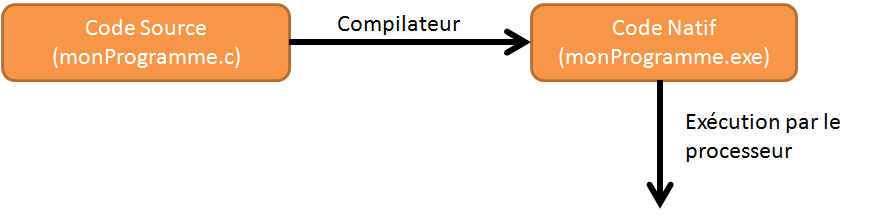
\includegraphics[scale=0.50]{images/comp_nat.png}
  \end{center}
\end{frame}

\begin{frame}
  \begin{center}
    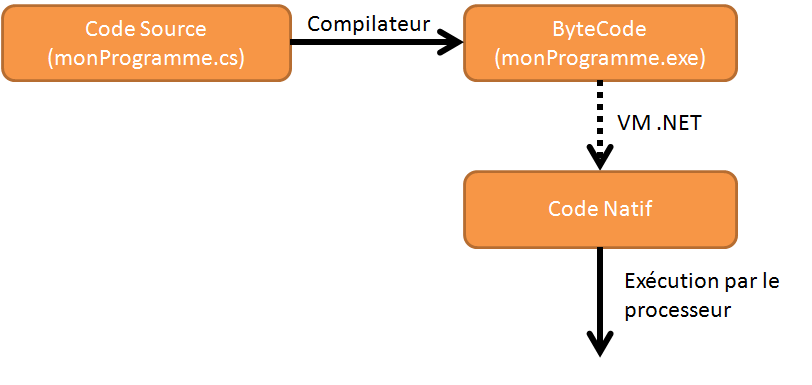
\includegraphics[scale=0.40]{images/comp_bc.png}
  \end{center}
\end{frame}

\section{Premier pas avec Visual Studio}

\begin{frame}
Live demo
\end{frame}


\section{L'imp\'eratif c'est quoi ?}
\subsection{Mon ordinateur, mon esclave}
\begin{frame}
  \begin{center}
    
\includegraphics[scale=0.35]{images/esclave.jpg}
  \end{center}
\end{frame}

\begin{frame}
    \begin{itemize}

	\item<1-> Fais moi un sandwich;
	\item<2-> Fais la vaisselle;
	\item<3-> Sors la poubelle;

	\item<4-> Tant que (le sol est sale): \\
	\{ Lave le sol; \} 

	\item<5-> Si (il y a du courrier):\\
	 \{Va chercher le courier; \} 
    \end{itemize}
\end{frame}

\section{Le langage CSharp}
\subsection{Les bases}
\begin{frame}
Les variables :
	\begin{itemize}
		\item<1-> \lstinline{int monAge = 21;}
		\item<2-> \lstinline{float monAge = 21.0f;}
		\item<3-> \lstinline{string monAge = "j'ai 21 ans";}
	\end{itemize}
\end{frame}


\begin{frame}[fragile]
Utiliser les variables :

 	\begin{center}
		\begin{lstlisting}
			int valueA = 10;
			valueA = 42;
		\end{lstlisting}
	\end{center}

 	\begin{center}
		\begin{lstlisting}
			int valueB = 40;
			valueB = valueB + 2;
		\end{lstlisting}
	\end{center}

 	\begin{center}
		\begin{lstlisting}
			string valueC = "Shugo";
			valueC = "Hello " + valueC + "!";
		\end{lstlisting}
	\end{center}

\end{frame}

\subsection{Les structures de controle}
\begin{frame}[fragile]
Le test:
		\begin{lstlisting}
			string myName = "Shugo";
			if (myName == "Shugo")
			{
 				console.writeLine("Hello Shugo");
			}
			else
			{
 				console.writeLine("I don't know you");
			}
		\end{lstlisting}

\end{frame}

\begin{frame}[fragile]
Le test:
		\begin{lstlisting}
			string myName = "Shugo";
			if (myName != "Shugo")
			{
 				console.writeLine("You are not Shugo");
			}
			else
			{
 				console.writeLine("You are Shugo");
			}
		\end{lstlisting}

\end{frame}

\begin{frame}[fragile]
La boucle for:
		\begin{lstlisting}
		for (int n = 0; n <  10; n++)
		{
 			console.writeLine(n);
		}
		\end{lstlisting}
\end{frame}

\begin{frame}[fragile]
La boucle while:
		\begin{lstlisting}
		int n = 0;
		while (n < 10)
		{
 			console.writeLine(n);
 			n = n + 1;
		}
		\end{lstlisting}
\end{frame}


\subsection{Tout est objet,  ma petite amie aussi ?}
\begin{frame}[fragile]
Utiliser les objets :
	\begin{center}
		\begin{lstlisting}
			Bitmap image = new Bitmap(512, 512);
			image.setPixel(10, 10, Color.White);
		\end{lstlisting}
	\end{center}
\end{frame}

\begin{frame}[fragile]
	\begin{table}
	\centering 
	\begin{tabular}{cc}
		\begin{tabular}{c}
\includegraphics[scale=0.10]{images/femme.png}\end{tabular} & 
		\begin{tabular}{c}\lstinputlisting{girlfriend_1.cs}\end{tabular}
	\end{tabular}
	\end{table}
\end{frame}

\begin{frame}[fragile]
	\begin{table}
	\centering 
	\begin{tabular}{cc}
		\begin{tabular}{c}
\includegraphics[scale=0.10]{images/femme.png}\end{tabular} & 
		\begin{tabular}{c}\lstinputlisting{girlfriend_2.cs}\end{tabular}
	\end{tabular}
	\end{table}
\end{frame}

\begin{frame}[fragile]
	\lstinputlisting{girlfriend_3.cs}

	\only<2->{My boyfriend is Kevin and he loves my boobs} 

	\only<3->{My boyfriend is Maxime and he loves my boobs}

\end{frame}

\begin{frame}[fragile]
        \lstinputlisting{vector.cs}
\end{frame}

\begin{frame}[fragile]
        \lstinputlisting{vector2.cs}
	\only<2->{X: 42 Y: 42} 
\end{frame}

\begin{frame}
Questions, remarques, choses pas claires ?
\end{frame}

\end{document}
